\documentclass{handout}
\SetHandoutTitle{Symplektische Verfahren und Schrittweitenkontrolle} %{Symplektische Verfahren mit variabler Zeitschrittweite}
\SetUniversitaet{Johannes Gutenberg-Universität Mainz}
\SetDatum{08.Mai.2024}
\SetFakultaet{Fachbereich 08}
\SetSemester{Sommersemester 2024}
\SetDozent{Prof. Dr. Hendrik Ranocha}
\SetReferent{Collin Wittenstein}
\SetSeminar{Numerik ODE}
\SetLiteratur{handout}

\hypersetup{
    pdftitle={Handout \HandoutTitle},
    pdfauthor={\Referent},
    pdfsubject={},
    pdfkeywords={},
    pdfcreator={LaTeX, hyperref, KOMA-Script}, % Ersteller
  }
\begin{document}
\maketitle

\section{Wiederholung Numerik ODE}
\subsection{Hamiltonsche Systeme}
Wir betrachten Hamiltonsche Systeme der folgenden Form
\begin{equation}
u^{\prime}(t)=J^{-1} H^{\prime}(u(t)),  \quad J=\left(\begin{array}{cc}
0 & \mathrm{I} \\
-\mathrm{I} & 0
\end{array}\right), \quad u(t) = \left(\begin{array}{c} p(t) \\ q(t) \end{array}\right)
\end{equation}
Wobei der Hamiltonien $H$ eine Erhaltungsgröße ist.

\subsection{Symplektisch}
Eine lineare Abbildung A heißt symplektisch, genau dann, wenn sie die Bilinearform $\langle \cdot,J\cdot\rangle$ erhält. Es also gilt:
\begin{equation}
    \langle Ax, J Ay\rangle = \langle x, J y\rangle \quad \forall x,y \in \mathbb{R}^{2d}.
\end{equation}
Eine differenzierbare Abbildung heißt symplektisch, genau dann, wenn ihre Jacobi-Matrix symplektisch ist. 

\subsection{Charakteristische Eigenschaften Hamiltonscher Systeme}

ODE Systeme $u^{\prime}(t)=f(u(t))$ sind genau dann (lokal) Hamiltonsch, wenn der zugehörige Fluss $\psi_t$ der $(p_0,q_0) \mapsto (p(t),q(t))$ abbildet, eine symplektische Abbildung ist. Zudem gilt dann, dass die differentielle 2-Form $dp\wedge dq$ erhalten bleibt.

\subsection{Symplektisches Verfahren}
Es kann kein numerisches Einschrittverfahren geben, welches beliebige Hamiltonien $H$ exakt erhält. Man kann jedoch Verfahren $\phi_h$ entwickeln, die $(p^n,q^n) \mapsto (p^{n+1},q^{n+1})$ symplektisch abbilden und damit die 2-Form $dp\wedge dq$ erhalten.

Symplektischen Verfahren besitzen viele Vorteile gegenüber klassischen Runge-Kutta-Verfahren, insbesondere wenn man über große Zeitskalen integriert. \cite{stackexchange} \cite{LectureODE}

\section{Numerisches Beispiele}
Diese Vorteile von symplektischen Verfahren werden schnell ersichtlich, wenn man folgendes Hamiltonsche System $\mathcal{H}=\frac{1}{2}\left(p_1^2+p_2^2\right)-\frac{1}{\sqrt{q_1^2+q_2^2}}$, welches den elliptischen Orbit eines Planeten um die Sonne modelliert, auf großen Zeitskalen betrachtet.

\begin{figure}[H]
    \centering
    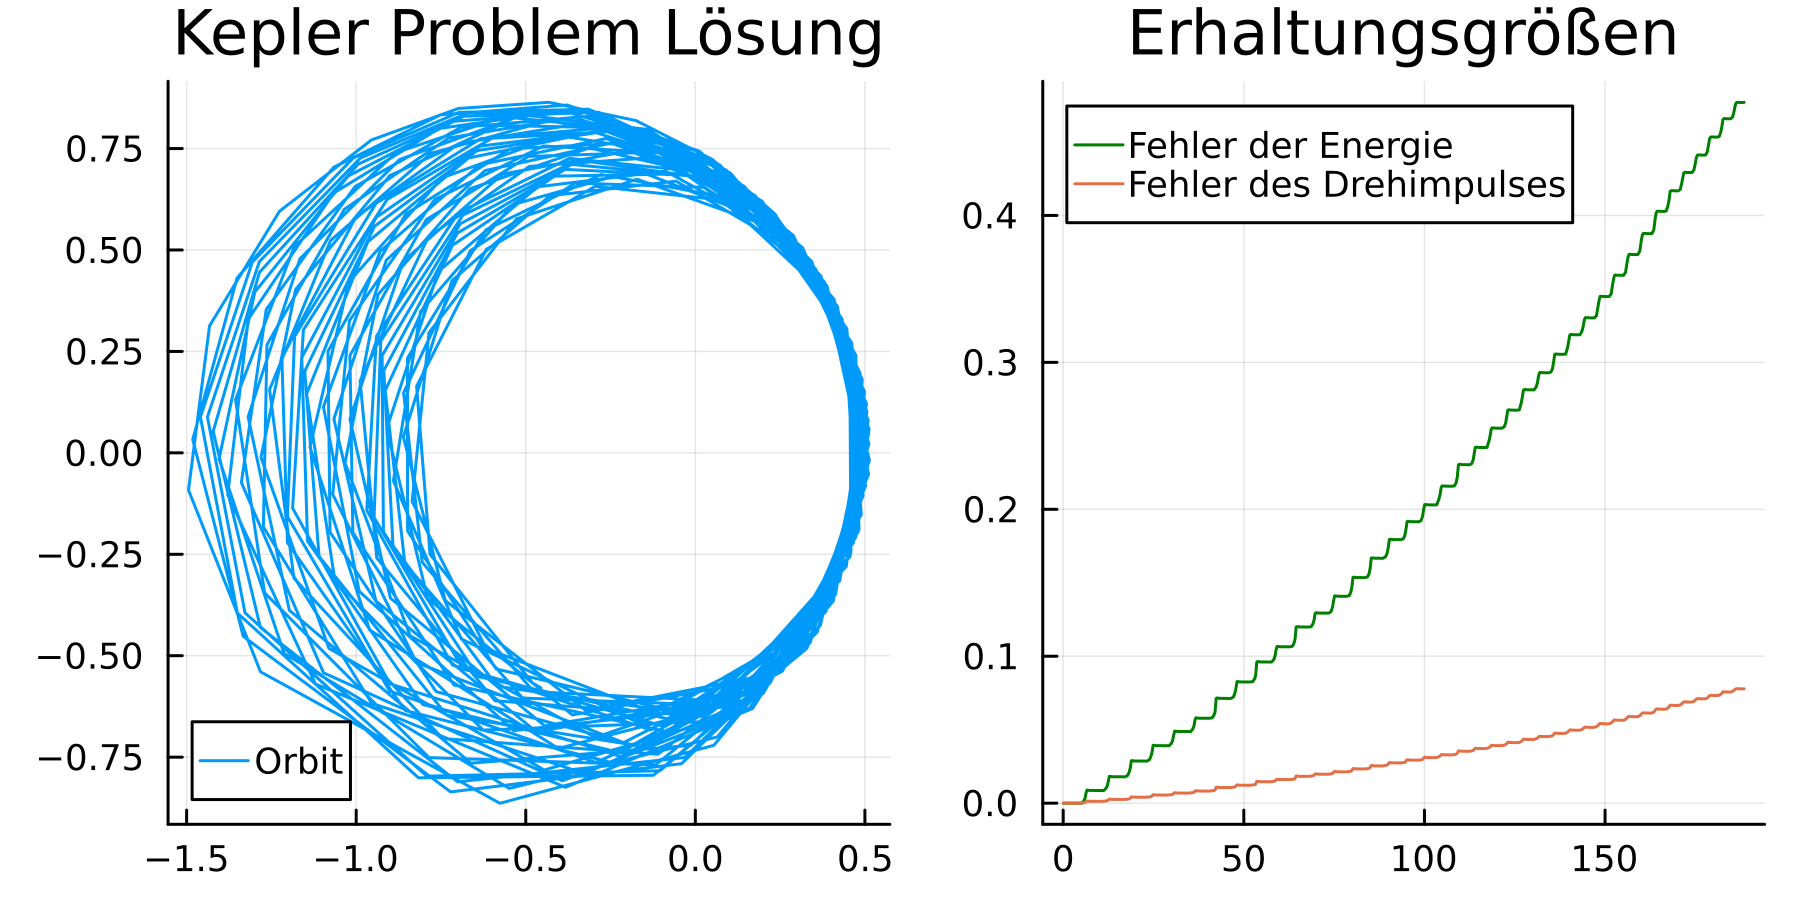
\includegraphics[scale = 0.20]{Tsit5.png}
    \caption{Zeitintegration über 30 Umläufe mithilfe des expliziten Runge-Kutta-Verfahrens Tsit5\centering}
    \label{fig:Tsit5}
\end{figure}

\begin{figure}[H]
    \centering
    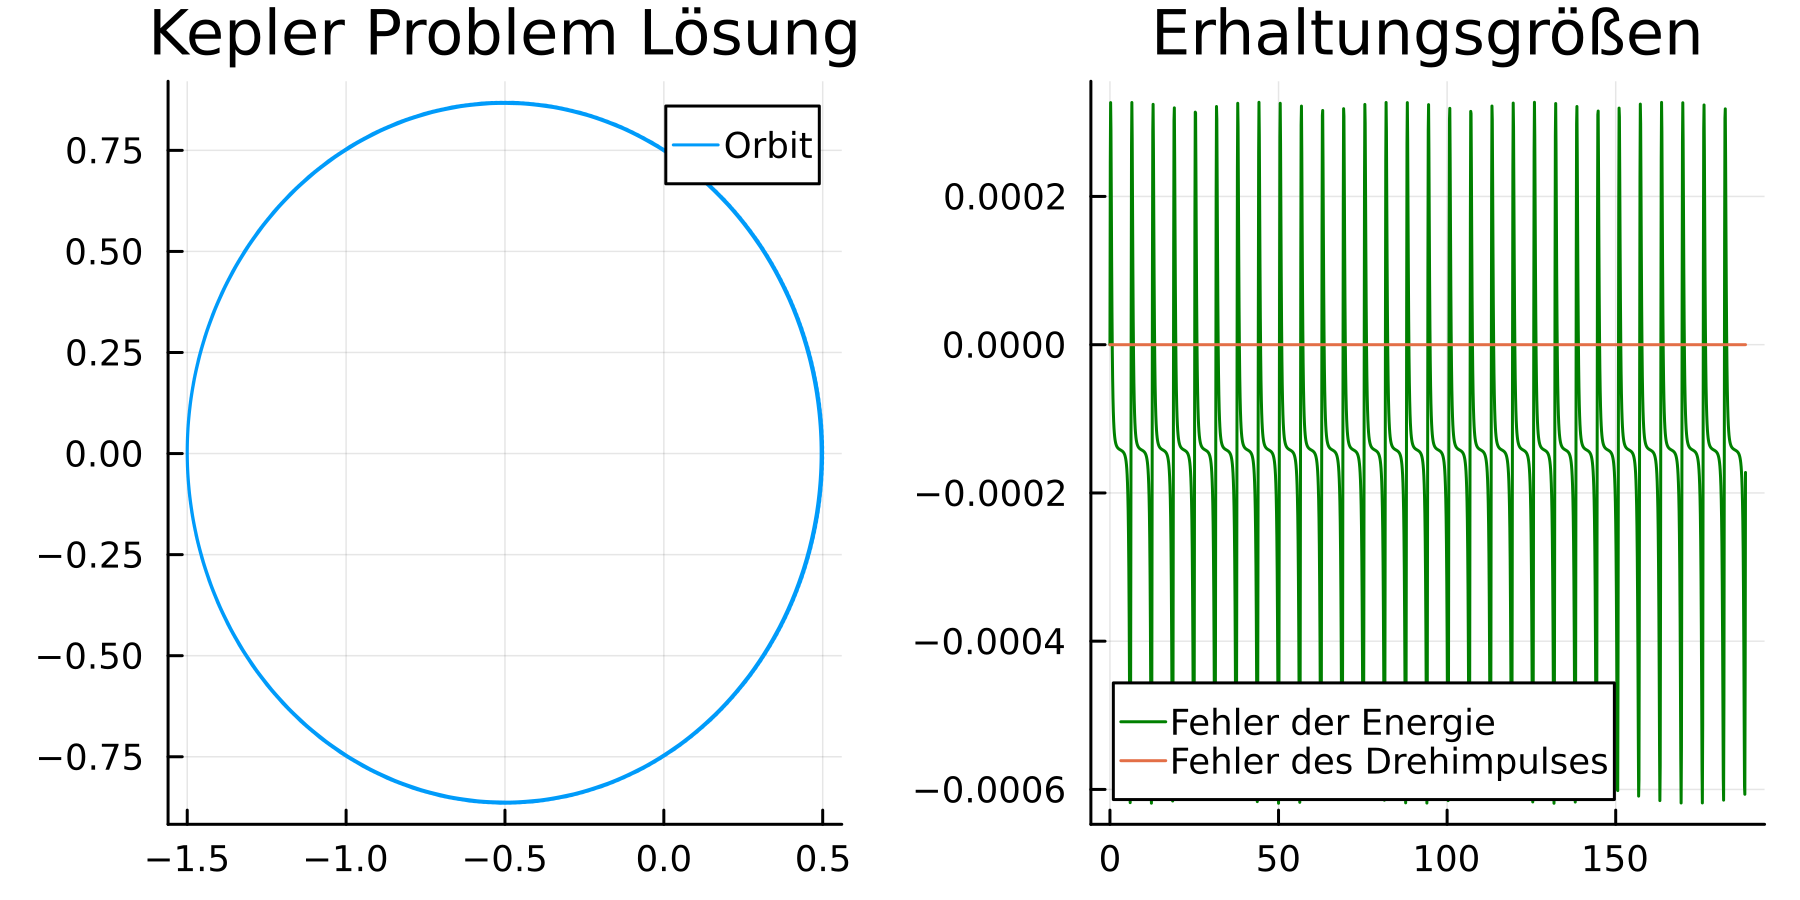
\includegraphics[scale = 0.20]{symp.png}
    \caption{Zeitintegration über 30 Umläufe mithilfe des symplektischen Verfahrens Ruth3\centering}
    \label{fig:symp}
\end{figure}

Während der Orbit des Planeten beim expliziten Verfahren langsam aber sicher der Sonne immer näher kommt und es zudem einen linearen Drift in der Gesamtenergie des Systems gibt, bleibt die Lösung des symplektische Verfahren auf der Umlaufbahn und die Gesamtenergie bleibt zwar nicht exakt erhalten, ihr Fehler ist aber periodisch. 

\section{Symplektische Verfahren und Schrittweitenkontrolle}
Ein wesentlicher Bestandteil von klassischen Runge-Kutta-Verfahren ist die Schrittweitenkontrolle. Mithilfe dieser können wir sicherstellen, dass unsere numerische Lösung im Rahmen unserer vorgebenden Toleranz genau ist und zudem effizient berechnet wird.

Es gilt jedoch, dass eine Einschrittverfahren $\phi_{h_n}$ mit variabler Schrittweite $h_n = h\cdot \Theta(p^n,q^n;h)$ nur dann symplektisch sein können, wenn gilt $\Theta(p^n,q^n;h) = \Theta(p^0,q^0;h) + \mathcal{O}(h^2)$. Also anders gesagt, die Schrittweite $h_n$ asymptotisch konstant ist. Also ist es nicht möglich bei einem symplektischen Verfahren die Zeitschrittweite adaptive zu variieren.  

Den Beweis dazu findet man im Paper \textit{Does variable step size ruin a symplectic integrator?} von R.D. Skeel und C.W. Gear \cite{SKEEL1992311}.

\section{Ausblick}
Eine alternative Lösung für dieses Problem besteht darin, unser Verfahren nicht adaptiv zu gestalten, sondern stattdessen unser Hamiltonsches System zu transformieren $H(p, q) \mapsto K(p, q, \varepsilon)$. Das Lösen des neuen Systems $K$ mit konstanter Schrittweite, sollte dann dem lösen des ursprünglichen Systems $H$ mit variabler Schrittweite entsprechen. 

Eine solche mögliche Transformation ist gegeben durch
\begin{equation}
    K(p, q, \varepsilon)=s(p, q, \varepsilon)\left(H(p, q)-H_0\right)
\end{equation}
wobei gilt $H_0 = H(p^0, q^0)$ und $s(p, q, \varepsilon) > 0 $ eine zustandsabhängige Funktion ist.

Die neuen Bewegungsgleichungen sind dann gegeben durch
\begin{equation}
\begin{split}
     p^{\prime}=-s(p, q, \varepsilon) H_q(p, q)-s_q(p, q, \varepsilon)\left(H(p, q)-H_0\right) \\
     q^{\prime}=s(p, q, \varepsilon) H_p(p, q)+s_p(p, q, \varepsilon)\left(H(p, q)-H_0\right).
\end{split}
\end{equation}

Die Lösung des neuen Hamiltonians $K(p, q, \varepsilon)$  $(P(t),Q(t))$ hängt dann mit der Lösung $(p(t),q(t))$ des ursprünglichen Hamiltonians $H(p, q)$ folgendermaßen zusammen
\begin{equation}
\begin{split}
    P(t)=p(\alpha(t, \varepsilon)), \quad Q(t)=q(\alpha(t, \varepsilon)) \\
    \text{wobei} \quad \alpha(t, \varepsilon)=\int_0^t s(P(\tau), Q(\tau), \varepsilon) \mathrm{d} \tau .
\end{split}
\end{equation}
Weitere Informationen und mögliche Probleme dieses Ansatz sind zu finden in dem Paper \textit{Variable time step integration with symplectic methods} von Ernst Hairer \cite{HAIRER1997219}.

\section*{Git-Repository}
Dieses Handout, sowie die in meinem Vortrag verwendeten Pluto Notebooks sind in folgendem Git-Repository zu finden: \href{https://github.com/cwittens/Hauptseminar_ODE}{https://github.com/cwittens/Hauptseminar\_ODE}.


\makeliteratur
Latex Vorlage übernommen von \href{https://github.com/MrBlackRocket/LaTeX-Handout-Vorlage}{https://github.com/MrBlackRocket/LaTeX-Handout-Vorlage}

\end{document}